\newpage
\section{Analisi dei rischi} \label{AnalisiDeiRischi}
	Per svolgere un progetto in maniera \gloss{efficiente} ed \gloss{efficace}, viene effettuata un'analisi preliminare dei rischi che potrebbero ostacolare il \gloss{processo} di sviluppo.
	È quindi fondamentale avere un piano di gestione di tali rischi, che permetta di reagire immediatamente in caso dovessero presentarsi, annullandone o limitandone i danni.\\
	I seguenti punti spiegano come è stato deciso di trattare i rischi:
	\begin{itemize}
		\item \textbf{Identificazione}: individuare i potenziali rischi che potrebbero presentarsi.
		\item \textbf{Analisi}: determinare la probabilità di occorrenza e comprenderne la criticità.
		\item \textbf{Pianificazione}: definire strategie che possano evitare i rischi precedentemente incontrati.
		\item \textbf{Controllo}: si monitorano e si revisionano i rischi affinché non si presentino nel corso del progetto.
		\item \textbf{Revisione}: dopo aver risolto eventuali rischi incontrati, si rivede la strategia utilizzata nel caso vengano individuate migliorie per la procedura. Se queste si rivelano più efficaci, vengono applicate.
	\end{itemize}

	\subsection{Valutazione}
	Per la valutazione dei rischi, viene utilizzato uno strumento di misura chiamato Qualitative Risk Assessment che ne considera i criteri quantitativi e qualitativi,
	assegnando a ciascuno un valore di gravità determinato dalla probabilità che il rischio possa avvenire e dalla gravità con cui esso influenza il progetto.
	% VEDI : https://www2.deloitte.com/content/dam/Deloitte/it/Documents/risk/Board%20Academy%20Corso%20C6%2020%20dic%202012%20SDA%20Bocconi.pdf
	Dato il numero non elevato di rischi, si è scelto di mettere solamente tre livelli di gravità e probabilità producendo quindi una matrice con nove elementi. In
	questo modo i rischi possono essere classificati in tre livelli di importanza:

	\begin{itemize}
		\item Basso
		\item Medio
		\item Alto
	\end{itemize}

	\begin{figure}[H]
		\centering
		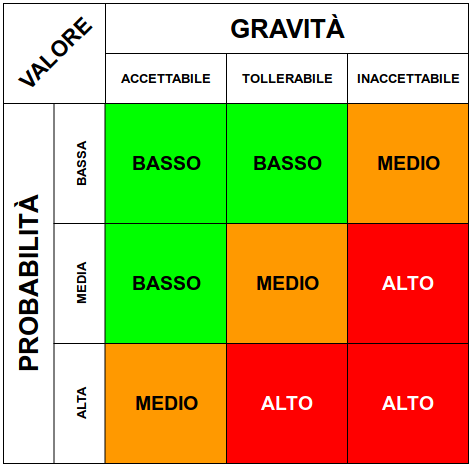
\includegraphics[scale=0.5]{img/risk_assessment_table.png}\\
		\caption{Matrice del Qualitative Risk Assessment}
		\label{fig:rischi}
	\end{figure}

	\subsection{Classificazione}

	A ciascun rischio viene assegnato un codice identificativo in modo da essere univoco e facilmente riconoscibile.

	Questo codice è:

	\begin{center}
		\texttt{[Tipologia][ID]-[Gravità][Probabilità][Classe]}
	\end{center}

	composto da:

	\begin{itemize}
		\item \textbf{Tipologia}:
			\begin{itemize}
				\item \textbf{O}: organizzativo.
				\item \textbf{P}: personale.
				\item \textbf{R}: requisiti.
				\item \textbf{S}: strumentale.
				\item \textbf{T}: tecnologico.
			\end{itemize}

		\item \textbf{ID}: numero progressivo di tre cifre che inizia da uno (001 - 999).
		\item \textbf{Gravità}:
			\begin{itemize}
				\item \textbf{0}: accettabile.
				\item \textbf{1}: tollerabile.
				\item \textbf{2}: inaccettabile.
			\end{itemize}

		\item \textbf{Probabilità}:
			\begin{itemize}
				\item \textbf{0}: bassa.
				\item \textbf{1}: media.
				\item \textbf{2}: alta.
			\end{itemize}

		\item \textbf{Classe}: ci si riferisce ai livelli di rischio individuati dalla matrice in Figura \ref{fig:rischi}
			\begin{itemize}
				\item \textbf{0}: basso (verde).
				\item \textbf{1}: medio (arancione).
				\item \textbf{2}: alto (rosso).
			\end{itemize}
	\end{itemize}

	Ad esempio, con P001-021 si può capire, seguendo la legenda, che si tratta del primo rischio del personale, di gravità accettabile, probabilità alta e un valore
	di classe medio.

	\subsection{Lista dei possibili rischi}

	Per elencare i rischi viene utilizzata una struttura tabellare che indica nella prima riga il codice identificativo e il nome di ciascun rischio,
	mentre nelle righe successive vengono elencate e discusse la relativa descrizione, le strategie per la rilevazione e le eventuali contromisure e mitigazioni.\par

%	Per elencare i rischi viene la seguente struttura tabellare:
%	\begin{table}[H]
%		\begin{risktable}{\columnwidth}{m{1.5cm}m{11.7cm}}
%			\thead{ID} &
%			\thead{Nome significativo}\\
%			\rowcolor{\tablegray}
%			\multicolumn{2}{X}{
%				\thead{Breve descrizione}
%			}\\
%			\multicolumn{2}{X}{
%				\thead{Strategie per la rilevazione}
%			}\\
%			\rowcolor{\tablegray}
%			\multicolumn{2}{X}{
%				\thead{Contromisure e mitigazione}
%			}\\
%		\end{risktable}
%		\caption[Analisi dei rischi]{Struttura della tabella dell'analisi dei rischi}
%	\end{table}

	Dopo un'attenta analisi del capitolato e alcuni incontri tra i componenti del team di sviluppo, è stato deciso di catalogare i seguenti rischi elencandoli in
	maniera crescente rispetto all'ID.
%	\mydoublerule{\linewidth}{0pt}{2pt}
	\begin{table}[H]
		\begin{risktable}{\columnwidth}{m{1.5cm}m{13.5cm}}
			\thead{P001-111} &
			Inesperienza del team a livello tecnico\\
			\rowcolor{\tablegray}
			\multicolumn{2}{X}{
				\textbf{Descrizione}: non tutti i componenti del team hanno le conoscenze di ambienti di sviluppo, linguaggi di programmazione e strumenti richiesti dall'azienda allo stesso livello.
			}\\
			\multicolumn{2}{X}{
				\textbf{Strategia}: sarà compito del \Res\ di progetto parlare con il resto del team di sviluppo e capire le conoscenze di ciascuna delle tecnologie che saranno utilizzate per lo sviluppo del progetto.
			}\\
			\rowcolor{\tablegray}
			\multicolumn{2}{X}{
				\textbf{Mitigazione}: ciascun componente si impegna a sanare le proprie lacune e a portarsi ad un livello comune concordato, in modo da poter lavorare autonomamente e potersi prendere impegni risolvibili senza dover usare tempo ulteriore per imparare la tecnologia.
			}\\
		\end{risktable}
		\caption{Specifica rischio P001-111}
	\end{table}

	\mydoublerule{\linewidth}{0pt}{2pt}

	\begin{table}[H]
		\begin{risktable}{\columnwidth}{m{1.5cm}m{13.5cm}}
			\thead{P002-122} &
			Impreparazione del team a livello gestionale \\
			\rowcolor{\tablegray}
			\multicolumn{2}{X}{
				\textbf{Descrizione}: non avendo affrontato progetti del genere prima d'ora, i componenti di \gruppo\ non conoscono bene i ruoli che devono intraprendere e i compiti da svolgere.
			}\\
			\multicolumn{2}{X}{
				\textbf{Strategia}: sarà compito di chi copre il ruolo di \Res\ assicurarsi che non ci siano perplessità da parte degli altri membri sui ruoli ricoperti e sui compiti assegnati.
			}\\
			\rowcolor{\tablegray}
			\multicolumn{2}{X}{
				\textbf{Mitigazione}: durante le ore di studio personale, ciascun componente si impegnerà a studiare la gerarchia dei ruoli\protect\footnotemark\ e, in caso di dubbi, ne parlerà con il team di sviluppo oppure direttamente con il \Res.
			}\\
		\end{risktable}
		\caption{Specifica rischio P002-122}
	\end{table}

	\footnotetext{Riferirsi alla voce
	%``Vincoli di \gloss{organigramma} e specifiche economiche''
	``3. Slide dell'insegnamento Ingegneria del software, Gestione di progetto'' 
	in \S\ref{rifnorma}}

	\mydoublerule{\linewidth}{0pt}{2pt}

	\begin{table}[H]
		\begin{risktable}{\columnwidth}{m{1.5cm}m{13.5cm}}
			\thead{P003-100} &
			Approvazione errata di documenti \\
			\rowcolor{\tablegray}
			\multicolumn{2}{X}{
				\textbf{Descrizione}: è possibile che il \Res\ commetta errori nell'approvazione dei documenti, che potrebbero portare alla consegna di documentazione errata o scadente, causando disguidi con il cliente e lasciando un'impressione negativa. \`E necessario correggere tali sviste, andando quindi a sprecare risorse investibili in altri compiti.
			}\\
			\multicolumn{2}{X}{
				\textbf{Strategia}: il \Res\ deve avere modo di controllare il lavoro prodotto dal proprio team in modo costante e graduale.
			}\\
			\rowcolor{\tablegray}
			\multicolumn{2}{X}{
				\textbf{Mitigazione}: colui che copre il ruolo di \Res\ deve assicurarsi che i documenti approvati siano effettivamente validi; in caso di sviste il \Ver\ deve saper trovare e correggere gli eventuali errori.
			}\\
		\end{risktable}
		\caption{Specifica rischio P003-100}
	\end{table}

%	\mydoublerule{\linewidth}{0pt}{2pt}

	\begin{table}[H]

		\begin{risktable}{\columnwidth}{m{1.5cm}m{13.5cm}}
			\thead{P004-100} &
			Cattiva gestione dell'archivio per la documentazione del progetto\\
			\rowcolor{\tablegray}
			\multicolumn{2}{X}{
				\textbf{Descrizione}: data la poca esperienza dei componenti del team di sviluppo con progetti di questo calibro, dove la documentazione è una delle parti principali, gestirla può risultare una novità e potrebbero presentarsi difficoltà nella gestione.
			}\\
			\multicolumn{2}{X}{
				\textbf{Strategia}: l'\Amm\ deve aver predisposto una \gloss{repository} comune in cui ciascun componente possa caricare il proprio lavoro, utilizzandola in maniera tale da non andare a modificare il lavoro caricato dagli altri.
			}\\
			\rowcolor{\tablegray}
			\multicolumn{2}{X}{
				\textbf{Mitigazione}: in caso di errori nella gestione della repository, l'\Amm\ deve saperli risolvere in maniera tempestiva, evitando che chi utilizzi successivamente la repository scarichi file errati, propagando l'errore anche sul proprio sistema.
			}\\
		\end{risktable}
		\caption{Specifica rischio P004-100}
	\end{table}

	\mydoublerule{\linewidth}{0pt}{2pt}

	\begin{table}[H]
		\begin{risktable}{\columnwidth}{m{1.5cm}m{13.5cm}}
			\thead{P005-021} &
			Intesa parziale tra i membri del team di sviluppo\\
			\rowcolor{\tablegray}
			\multicolumn{2}{X}{
				\textbf{Descrizione}: il team di sviluppo è formato principalmente da persone che precedentemente non si conoscevano o che hanno avuto poche interazioni tra di loro fino al momento della creazione di quest'ultimo.
				La mancata conoscenza delle competenze altrui potrebbe causare un'errata gestione del lavoro e dell'assegnazione dei compiti.
			}\\
			\multicolumn{2}{X}{
				\textbf{Strategia}: attraverso gli incontri diretti o con strumenti di chat quali \gloss{Slack}, ci si confronta e si realizzano i diversi modi di lavorare per ognuno.
			}\\
			\rowcolor{\tablegray}
			\multicolumn{2}{X}{
				\textbf{Mitigazione}: il team di sviluppo si impegna a conoscersi nel corso delle riunioni e ritrovi.
				Si discute insieme di un way of working comune che possa soddisfare le metodologie di lavoro di tutti i componenti.
				Nel caso in cui nascano dibattiti o sia difficile raggiungere un punto d'intesa, la decisione è presa dalla maggioranza.
				%e democrazia sia... purtroppo
				%In caso ci fossero dibattiti, per non ricorrere alle lame, gli altri componenti andranno a calmare le acque senza che ci siano morti.
				%LOOOL
			}\\
		\end{risktable}
		\caption{Specifica rischio P005-021}
	\end{table}

%	\mydoublerule{\linewidth}{0pt}{2pt}

	\begin{table}[H]

		\begin{risktable}{\columnwidth}{m{1.5cm}m{13.5cm}}
			\thead{P006-122} &
			Cattiva amministrazione delle risorse \\
			\rowcolor{\tablegray}
			\multicolumn{2}{X}{
				\textbf{Descrizione}: data l'inesperienza del team di sviluppo con progetti di questa natura, è possibile che sorgano problemi nell'amministrazione delle risorse come tempo, costi e suddivisione dei ruoli.
			}\\

			\multicolumn{2}{X}{
				\textbf{Strategia}: a ciascuna riunione di \gruppo, si controllerà se il lavoro svolto fino a quel momento è pertinente a quanto è stato preventivato, modificando di conseguenza il consuntivo e il \gloss{preventivo} a finire.
				Tramite strumenti come diagrammi di \gloss{Gantt} dinamici, dove ciascun componente può aggiornare i tempi previsti per completare l'attività assegnata, è possibile monitorare costantemente il progresso del progetto in modo tale da evitare situazioni di \gloss{zero laxity}.
			}\\

			\rowcolor{\tablegray}
			\multicolumn{2}{X}{
				\textbf{Mitigazione}: in caso dovessero sorgere problemi di questa natura, \gruppo\ si impegnerà a ridistribuire le risorse in modo da rispettare la tabella di marcia e in particolar modo le scadenze, tenendo conto di consegnare comunque un prodotto di \gloss{qualità}.
			}\\
		\end{risktable}
		\caption{Specifica rischio P006-122}
	\end{table}

	\mydoublerule{\linewidth}{0pt}{2pt}

	\begin{table}[H]
		\begin{risktable}{\columnwidth}{m{1.5cm}m{13.5cm}}
			\thead{O001-201} &
			Ritardo consegna del materiale per una revisione oltre la scadenza \\
			\rowcolor{\tablegray}
			\multicolumn{2}{X}{
				\textbf{Descrizione}: è possibile che uno o più componenti del team di sviluppo, per impegni legati alla propria vita privata o universitaria, non riescano a gestire i compiti assegnati, arrivando a una scadenza senza aver finito il proprio lavoro e obbligando l'intero team di sviluppo a rinviare la consegna.
			}\\

			\multicolumn{2}{X}{
				\textbf{Strategia}: sarà compito del \Res\ assicurarsi che il lavoro proceda in maniera lineare ponendo scadenze intermedie, monitorando il lavoro del team di sviluppo, organizzando riunioni e aggiornandosi sullo stato dei vari compiti assegnati secondo il way of working scelto.
			}\\

			\rowcolor{\tablegray}
			\multicolumn{2}{X}{
				\textbf{Mitigazione}: ciascun membro si impegna a gestire il proprio tempo adeguatamente in rapporto con gli altri impegni universitari senza trascurare il suo ruolo nel team di sviluppo, distinguendo le priorità in modo da non influenzare negativamente lo sviluppo del progetto. In caso di impegni che possano ostacolare questo obiettivo, ci si prenderà cura di avvisare gli altri componenti del team di sviluppo per tempo.
			}\\
		\end{risktable}
		\caption{Specifica rischio O001-201}
	\end{table}

	\mydoublerule{\linewidth}{0pt}{2pt}

	\begin{table}[H]
		\begin{risktable}{\columnwidth}{m{1.5cm}m{13.5cm}}
			\thead{O002-010} &
			Mancanza di comunicazione con l'azienda \\

			\rowcolor{\tablegray}
			\multicolumn{2}{X}{
				\textbf{Descrizione}: durante lo sviluppo del progetto, è possibile non riuscire a contattare i rappresentanti dell'azienda e che essi quindi non siano al corrente dei progressi fatti, dei requisiti completati e del modo in cui il team sta lavorando.
			}\\

			\multicolumn{2}{X}{
				\textbf{Strategia}: è opportuno che il \Res\ si metta in comunicazione con l'azienda, attraverso \gloss{Telegram}, \gloss{Hangouts} o tramite incontri di persona e riferisca il progresso svolto dal team di sviluppo, in modo da avere feedback e critiche costruttive che possano migliorare lo sviluppo del progetto.
			}\\

			\rowcolor{\tablegray}
			\multicolumn{2}{X}{
				\textbf{Mitigazione}: in caso di mancata comunicazione per un lungo arco di tempo, è opportuno che alla prima scadenza di revisione utile il team di sviluppo si impegni a contattare l'azienda per avere un suo feedback.
			}\\
		\end{risktable}
		\caption{Specifica rischio O002-010}
	\end{table}

	\mydoublerule{\linewidth}{0pt}{2pt}

	\begin{table}[H]
		\begin{risktable}{\columnwidth}{m{1.5cm}m{13.5cm}}
			\thead{S001-100} &
			Problematiche hardware \\

			\rowcolor{\tablegray}
			\multicolumn{2}{X}{
				\textbf{Descrizione}: è possibile che i computer e altri strumenti hardware che possono essere utilizzati dai membri del team di sviluppo risultino difettosi o smettano di funzionare.
			}\\

			\multicolumn{2}{X}{
				\textbf{Strategia}: ciascun membro avrà cura degli strumenti a sua disposizione in modo tale che non sorgano problemi che possano ostacolare il lavoro.
			}\\

			\rowcolor{\tablegray}
			\multicolumn{2}{X}{
				\textbf{Mitigazione}: i guasti di natura hardware non sono facilmente prevedibili, ma in caso dovessero presentarsi è possibile utilizzare temporaneamente i computer forniti dai laboratori dell'università fino a quando la macchina difettosa non venga riparata o, se necessario, sostituita.
			}\\
		\end{risktable}
		\caption{Specifica rischio S001-100}
	\end{table}

	\mydoublerule{\linewidth}{0pt}{2pt}

	\begin{table}[H]

		\begin{risktable}{\columnwidth}{m{1.5cm}m{13.5cm}}
			\thead{R001-122} &
			Interpretazione errata dei requisiti: aggiunta o modifica di requisiti in corso di sviluppo \\

			\rowcolor{\tablegray}
			\multicolumn{2}{X}{
				\textbf{Descrizione}: durante il progetto, dopo aver effettuato una prima analisi di tutti i requisiti, potrebbe sorgere il bisogno di modificare un requisito già fissato o aggiungerne uno non identificato in precedenza.
			}\\

			\multicolumn{2}{X}{
				\textbf{Strategia}: è possibile che nel corso dello sviluppo del progetto vengano scoperti requisiti secondari impliciti non precedentemente valutati che necessitino di essere sviluppati.
				A ciascuna milestone, anche intermedia, è utile controllare che la lista dei requisiti da svolgere sia coerente con quella richiesta dall'azienda, analizzando il documento che presenta il loro capitolato.
			}\\

			\rowcolor{\tablegray}
			\multicolumn{2}{X}{
				\textbf{Mitigazione}: nel caso dovesse sorgere la necessità di sviluppare requisiti non previsti, questi andranno analizzati per capire di che risorse hanno bisogno e come andranno inseriti nella scaletta di sviluppo del progetto in modo adeguato. Data la natura modulare del progetto, ciascun requisito verrà sviluppato in ordine di importanza, in modo da dover svolgere compiti facilmente monitorabili e testabili.
			}\\
		\end{risktable}
		\caption{Specifica rischio R001-122}
	\end{table}

	%\mydoublerule{\linewidth}{0pt}{2pt}

	\begin{table}[H]

		\begin{risktable}{\columnwidth}{m{1.5cm}m{13.5cm}}
			\thead{T001-100} &
			Problematiche software\\

			\rowcolor{\tablegray}
			\multicolumn{2}{X}{
				\textbf{Descrizione}: il team di sviluppo fa affidamento a prodotti software per l'integrazione del codice e dei documenti. Eventuali problemi possono causare gravi perdite di dati.
			}\\

			\multicolumn{2}{X}{
				\textbf{Strategia}: siccome ci si affida a servizi di terze parti, i malfunzionamenti che potrebbero capitare sono imprevedibili, ma data la nota affidabilità di questi strumenti, la probabilità che questo rischio insorga è molto bassa.
			}\\

			\rowcolor{\tablegray}
			\multicolumn{2}{X}{
				\textbf{Mitigazione}: ciascun componente si impegna a mantenere una copia, aggiornata periodicamente, della repository contenente i file di progetto, nella propria macchina o eventualmente in una memoria esterna.
			}\\
		\end{risktable}
		\caption{Specifica rischio T001-100}
	\end{table}
